\documentclass{standalone}
\usepackage{pgfplots}
\pgfplotsset{compat=1.17}

\begin{document}

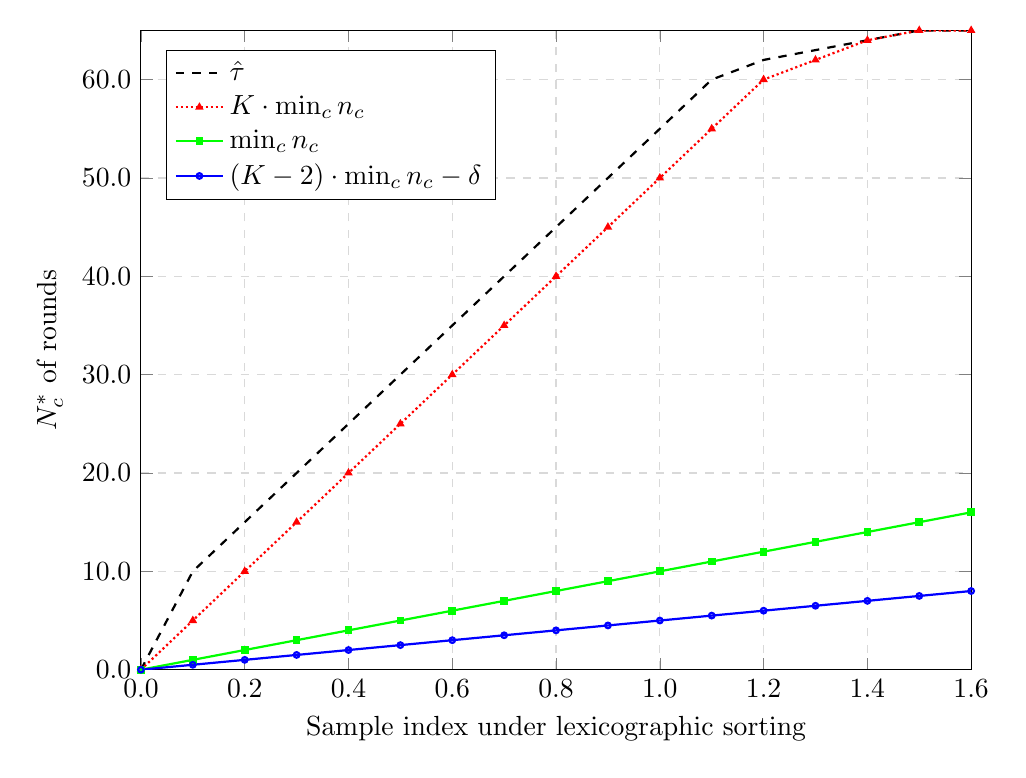
\begin{tikzpicture}
    \begin{axis}[
        width=\textwidth,
        height=0.8\textwidth,
        xlabel={Sample index under lexicographic sorting},
        ylabel={$N_c^*$ of rounds},
        xmin=0, xmax=1.6,
        ymin=0, ymax=65,
        xtick={0,0.2,...,1.6},
        ytick={0,10,...,60},
        legend pos=north west,
        legend cell align=left,
        grid=major,
        grid style={dashed, gray!30},
        ticklabel style={/pgf/number format/.cd, fixed, fixed zerofill, precision=1},
        every axis plot post/.append style={
            thick,
            mark size=1pt,
            mark options={solid},
        },
    ]

        % Black line (\hat{\tau})
        \addplot+[black, dashed, no marks] table {
            x y
            0   0
            0.1 10
            0.2 15
            0.3 20
            0.4 25
            0.5 30
            0.6 35
            0.7 40
            0.8 45
            0.9 50
            1.0 55
            1.1 60
            1.2 62
            1.3 63
            1.4 64
            1.5 65
            1.6 65
        };
        \addlegendentry{$\hat{\tau}$};

        % Red dotted line (K * min_c n_c)
        \addplot+[red, densely dotted, mark=triangle*, mark options={rotate=180}] table {
            x y
            0   0
            0.1 5
            0.2 10
            0.3 15
            0.4 20
            0.5 25
            0.6 30
            0.7 35
            0.8 40
            0.9 45
            1.0 50
            1.1 55
            1.2 60
            1.3 62
            1.4 64
            1.5 65
            1.6 65
        };
        \addlegendentry{$K \cdot \min_c n_c$};

        % Green solid line (min_c n_c)
        \addplot+[green, solid, mark=square*] table {
            x y
            0   0
            0.1 1
            0.2 2
            0.3 3
            0.4 4
            0.5 5
            0.6 6
            0.7 7
            0.8 8
            0.9 9
            1.0 10
            1.1 11
            1.2 12
            1.3 13
            1.4 14
            1.5 15
            1.6 16
        };
        \addlegendentry{$\min_c n_c$};

        % Blue solid line ((K-2) * min_c n_c - \delta)
        \addplot+[blue, solid, mark=o] table {
            x y
            0   0
            0.1 0.5
            0.2 1
            0.3 1.5
            0.4 2
            0.5 2.5
            0.6 3
            0.7 3.5
            0.8 4
            0.9 4.5
            1.0 5
            1.1 5.5
            1.2 6
            1.3 6.5
            1.4 7
            1.5 7.5
            1.6 8
        };
        \addlegendentry{$(K-2) \cdot \min_c n_c - \delta$};

    \end{axis}
\end{tikzpicture}

\end{document}